%%==================================================================%%
%% Author : Sa�udo Olmedo, Ignacio                                  %%
%%          S�nchez Barreiro, Pablo                                 %%
%% Version: 1.2, 18/06/2014                                         %%
%%                                                                  %%
%% Memoria del Proyecto Fin de Carrera                              %%
%% Planificacion/CasoEstudio                                        %%
%%==================================================================%%

\begin{figure}[!tb]
  \centering
  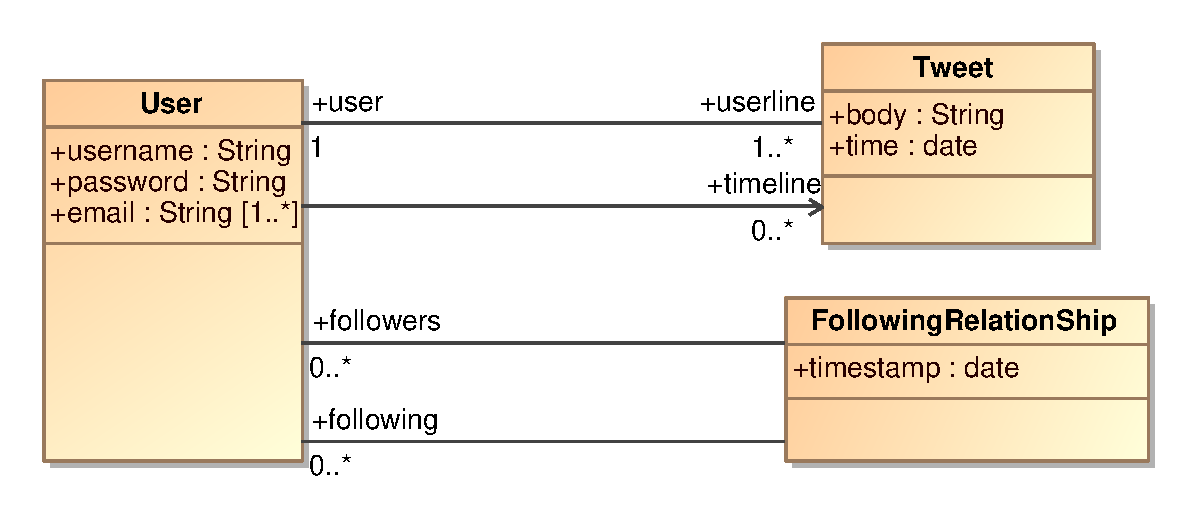
\includegraphics[width=.8\linewidth]{m2m/images/twissandra.eps} \\
  \caption{Modelo UML Twissandra}
  \label{back:fig:twissandra}
\end{figure}

Esta secci�n presenta \emph{Twissandra}, el caso de estudio que se utilizar� lo largo de este proyecto. Twissandra es un proyecto creado para aprender como utilizar Cassandra. El modelo UML correspondiente a Twissandra se puede ver en la figura~\ref{back:fig:twissandra}. Twissandra es una versi�n simplificada de Twitter.

Twitter\footnote{} es una red social de microblogging, actualmente est� muy extendida, que permite escribir a sus usuarios peque�os mensajes de texto, denominados \emph{tweets}. Un \emph{tweet} es simplemente un texto con un l�mite de 140 caracteres publicado a una hora determinada. La colecci�n de todos los tweets publicados por un usuario cronol�gicamente ordenados determinan su \emph{userline}.

Cada usuario registrado en Twitter puede seguir a otros usuarios registrados. Cuando decimos, por ejemplo, que Pedro sigue a Mar�a significa que Pedro recibir� en su cuenta todos los mensajes que publique Mar�a. En este caso, se dice que Pedro es un \emph{follower} de Mar�a. De esta forma, cada usuario tiene asociado un \emph{timeline} que no es m�s que la colecci�n de todos los \emph{tweets} publicados por las personas a las que sigue ordenados cronol�gicamente, es decir, por fecha de publicaci�n. 

Los principales casos de uso de \emph{Twissandra} son: 

\begin{enumerate}
    \item Obtener el \emph{timeline} de un usuario determinado. 
    \item Obtener el \emph{userline} de un usuario determinado. 
    \item Obtener la lista de usuarios que un usuario est� siguiendo.  
    \item Obtener la lista de usuarios que est�n siguiendo a un usuario espec�fico. 
\end{enumerate}

Las dos �ltimas listas deben se deben devolver ordenadas cronol�gicamente.

%%========================================================================================%%
%% NOTA(Pablo): Esta justificaci�n es d�bil, as� que mejor quitarla                       %%
%%========================================================================================%%

Como vemos \imp{Twissandra} es una versi�n simplificada de Twitter. Sin embargo, se considera un buen ejemplo a analizar ya que Twitter goza de gran popularidad y es una de las redes sociales m�s usadas del mundo. 

Una vez entendido esto en los siguientes cap�tulos se procede a detallar el proceso de creaci�n de un repositorio de datos en Cassandra que cubra los casos de usos citados anteriormente describiendo los procesos de transformaci�n entre modelos que se realizaran as� como la generaci�n de c�digo del repositorio de datos en Twissandra.
